\begin{frame}{Generalization}
  \begin{figure}
    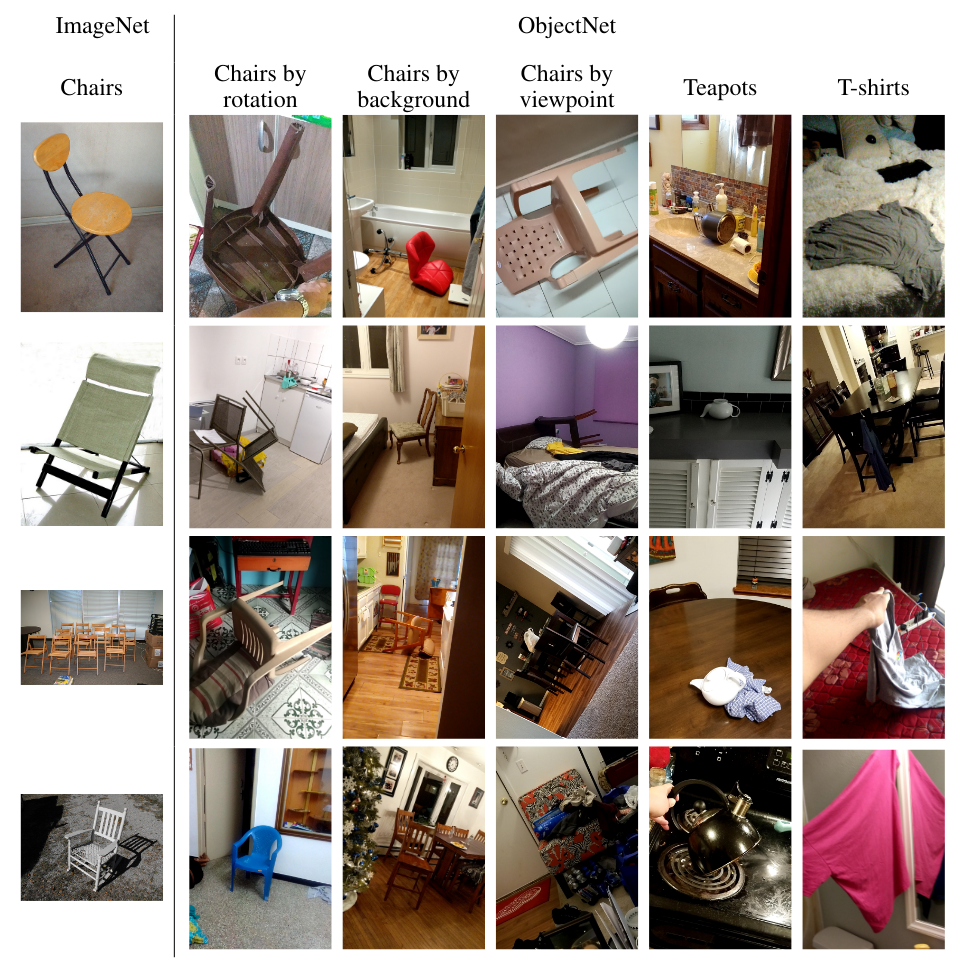
\includegraphics[width=0.4\textwidth]{objectnet_examples}
    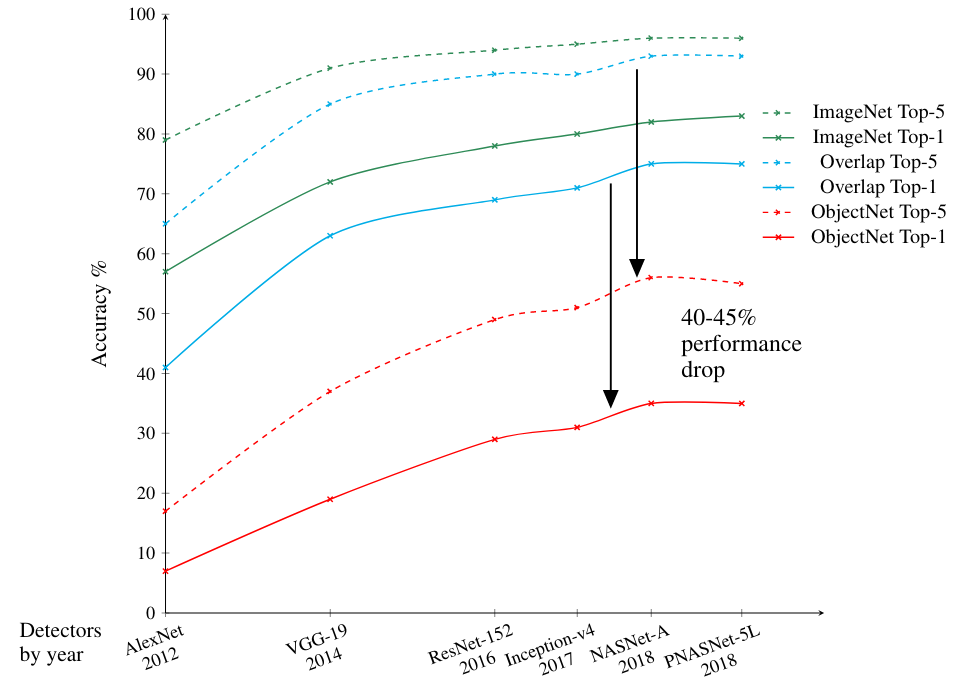
\includegraphics[width=0.55\textwidth]{objectnet_graph}
  \end{figure}

  \note{
    \begin{itemize}
      \item Neural Networks trained and evaluated on ImageNet do not generalize to o.o.d. data.
      \item Image from ObjectNet: A large-scale bias-controlled dataset forpushing the limits of object recognition models, Barbu et al, NeurIPS 2019
    \end{itemize}
  }
\end{frame}


\begin{frame}{Neural Networks are lazy}
  \begin{figure}
    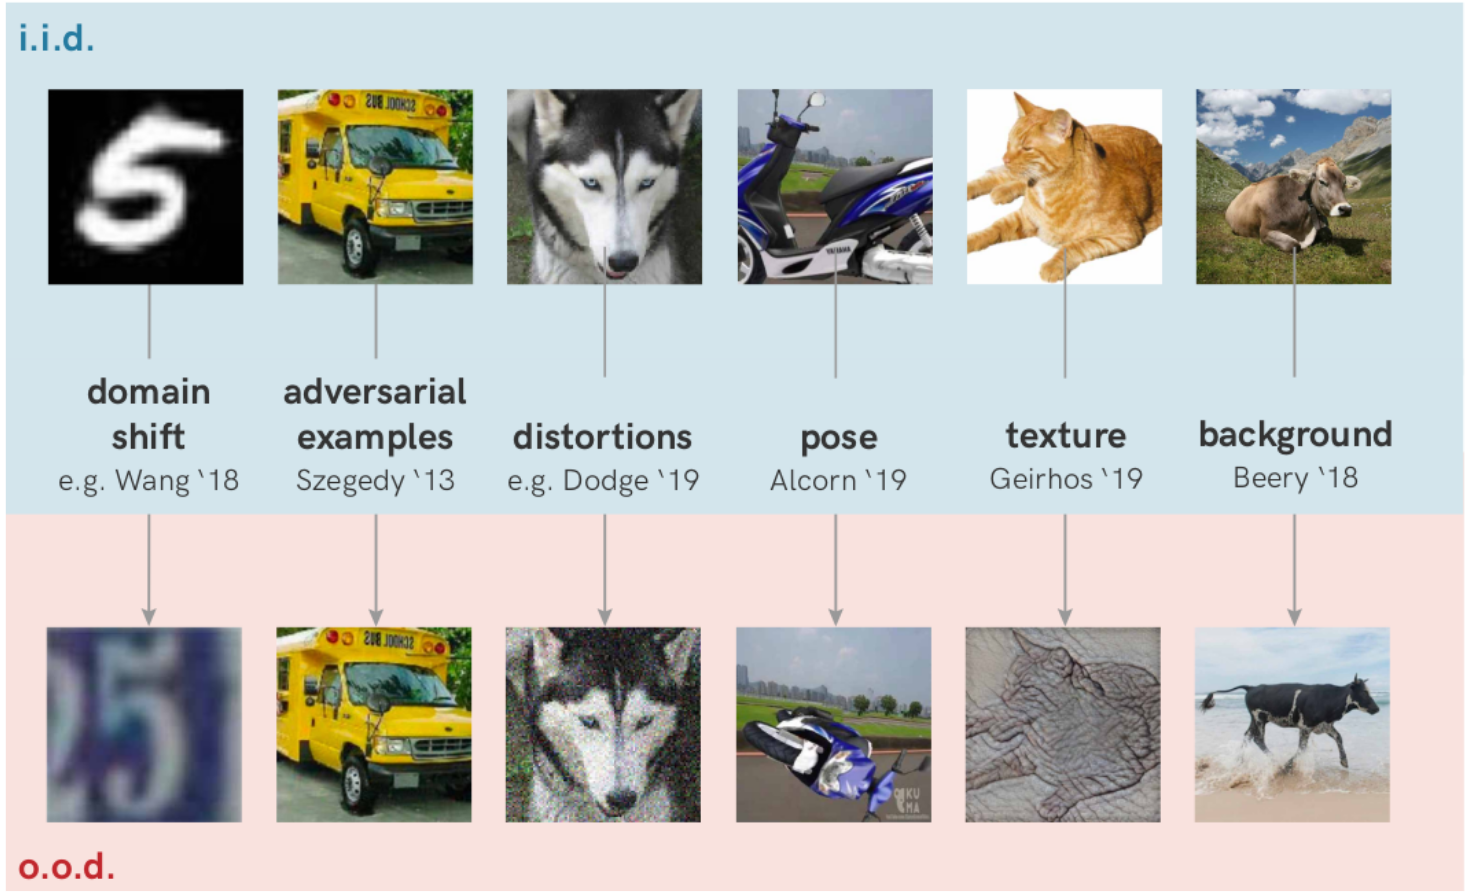
\includegraphics[width=0.9\textwidth]{shortcuts_00}
  \end{figure}

  \note{
    \begin{itemize}
      \item They learn shortcuts if we let them.
      \item Image from Shortcut Learning in Deep Neural Networks, Geirhos et al, Nature Machine Intelligence 2020
    \end{itemize}
  }
\end{frame}


\begin{frame}{Neural Networks are lazy}
  \begin{figure}
    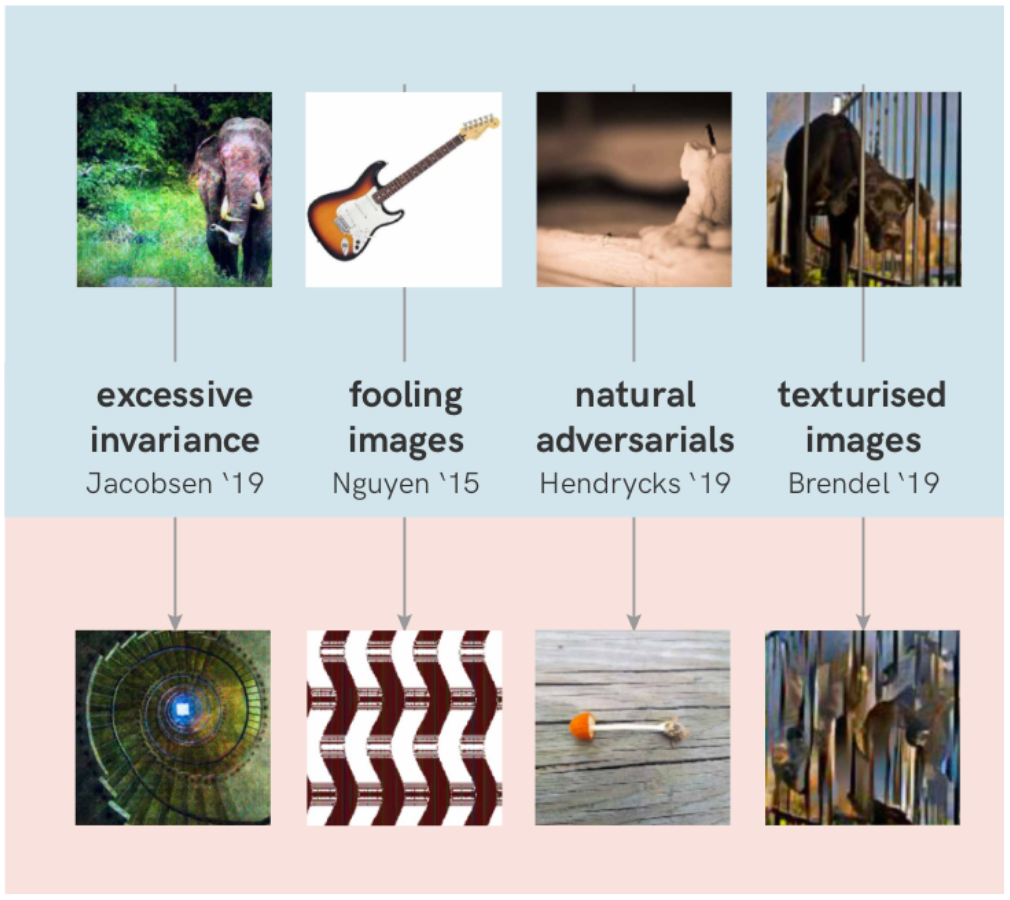
\includegraphics[width=0.6\textwidth]{shortcuts_01}
  \end{figure}

  \note{
    \begin{itemize}
      \item
      \item
      \item Image from Shortcut Learning in Deep Neural Networks, Geirhos et al, Nature Machine Intelligence 2020
    \end{itemize}
  }
\end{frame}


\begin{frame}{Investigate decisions: partial occlusion}
  \begin{figure}
    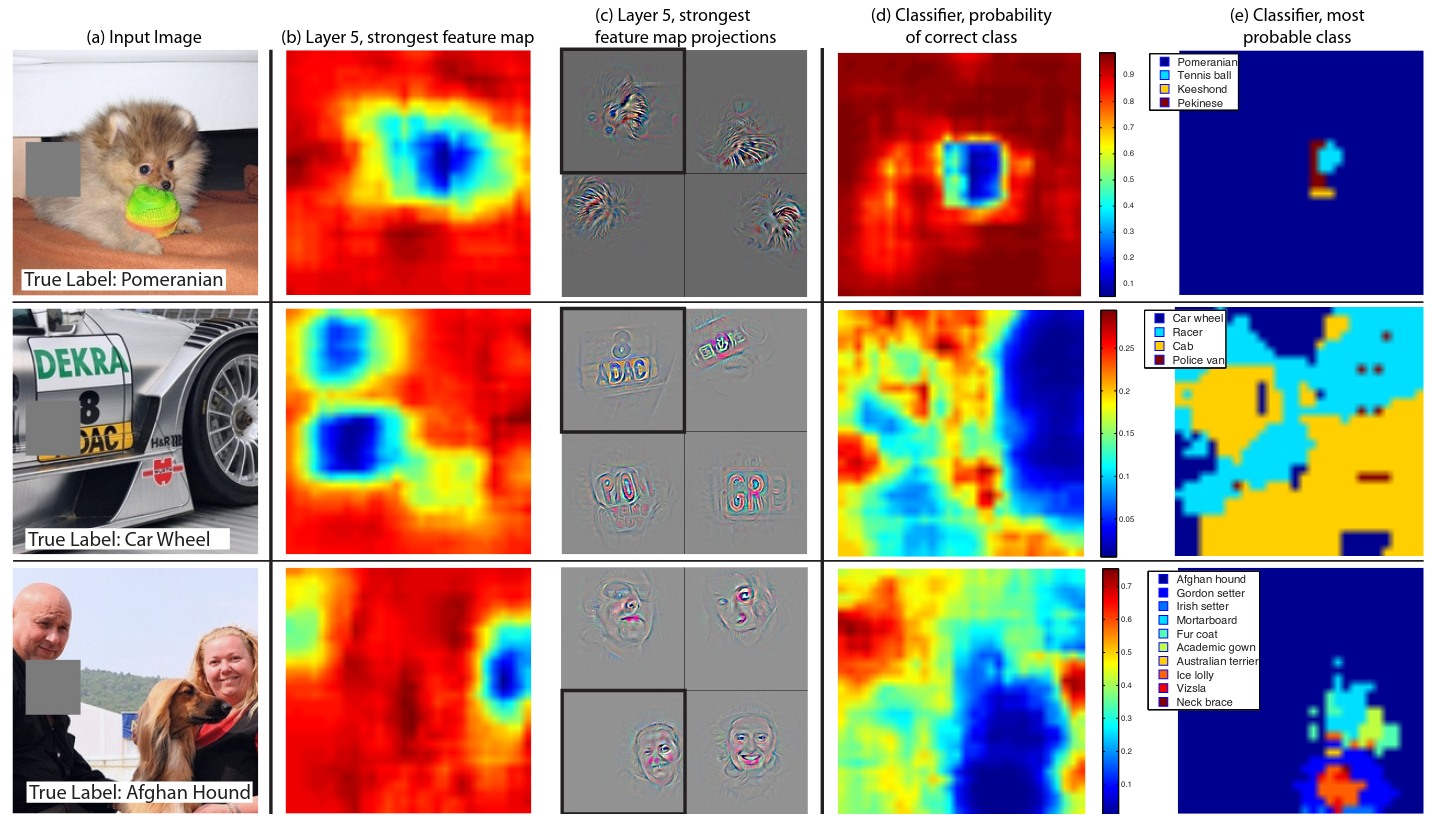
\includegraphics[width=0.9\textwidth]{occlusion}
  \end{figure}

  \note{
    \begin{itemize}
      \item An easy way for an visual sanity check is occluding parts of the image while watching the accuracy.
      \item Image from Visualizing and Understanding Convolutional Networks, Zeiler \& Fergus, ECCV 2014
    \end{itemize}
  }
\end{frame}


\begin{frame}{Investigate decisions: image gradient}
  \begin{figure}
    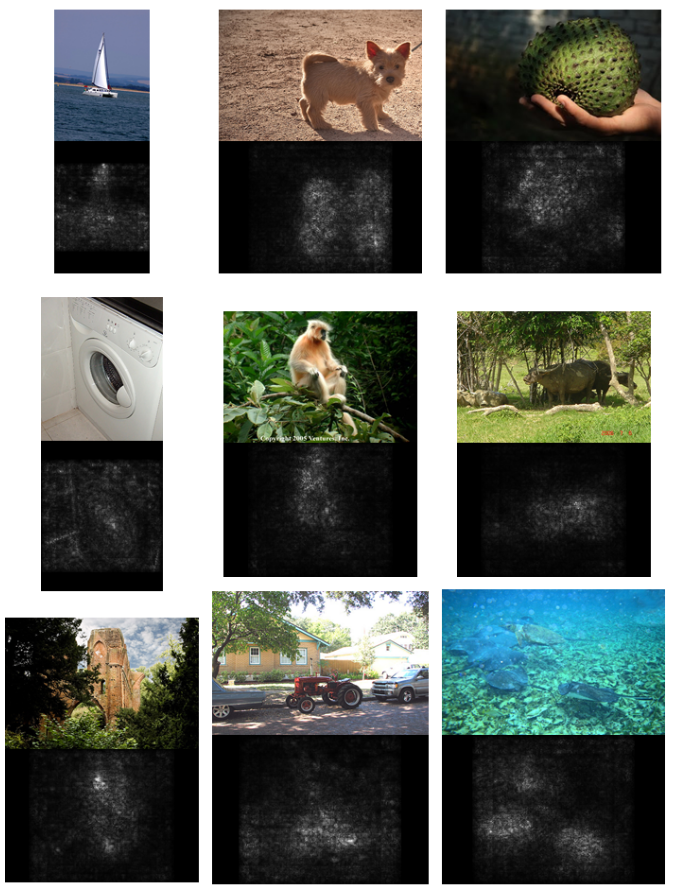
\includegraphics[width=0.4\textwidth]{image_backprop}
  \end{figure}

  \note{
    \begin{itemize}
      \item Looking at the pixel gradient of the network gives some insights too.
      \item Image from Deep Inside Convolutional Networks: Visualising Image Classification Models and Saliency Maps, Simonyan et al, 2013
    \end{itemize}
  }
\end{frame}


\begin{frame}{Investigate decisions: relevance propagation}
  \begin{figure}
    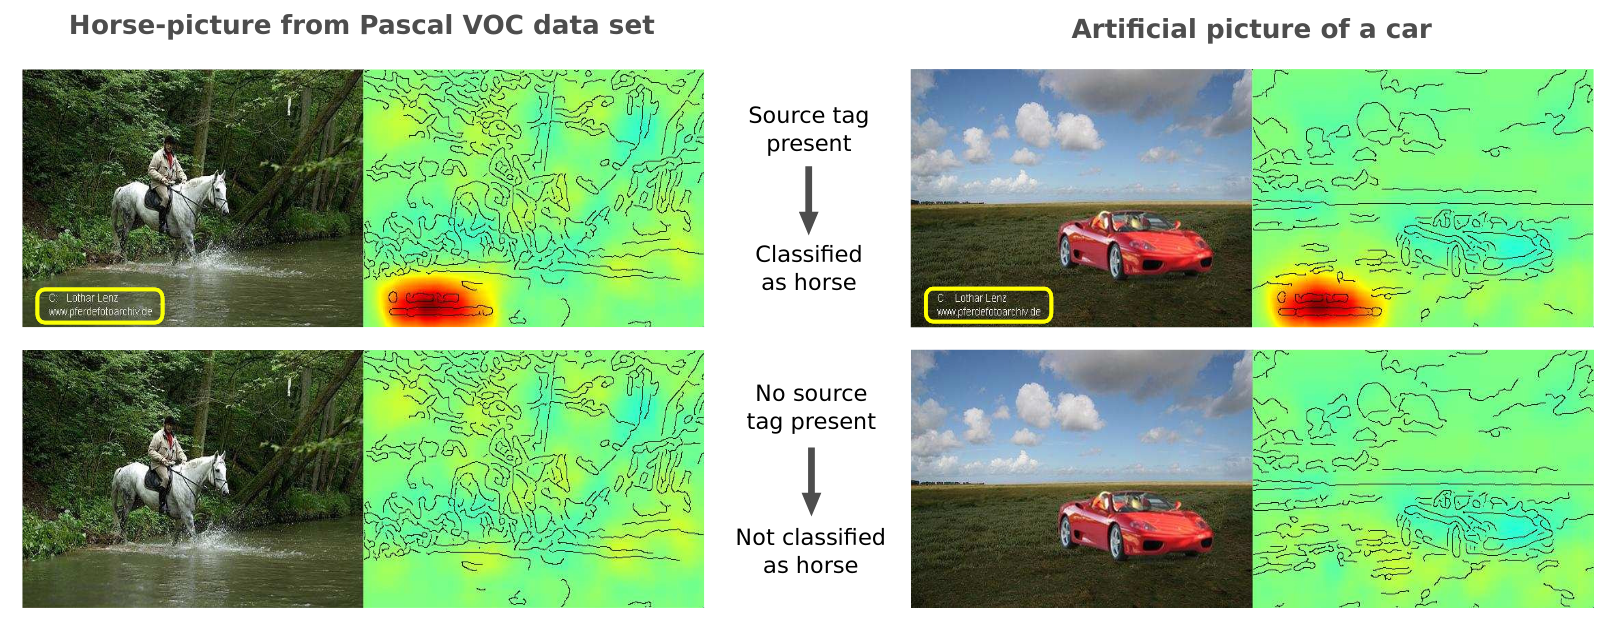
\includegraphics[width=0.9\textwidth]{relevance_propagation}
  \end{figure}

  \note{
    \begin{itemize}
      \item Explain the output, not the local variation.
      \item Image from Unmasking Clever Hans Predictors and Assessing What Machines Really Learn, Lapuschkin et al, Nature Communications 2019
    \end{itemize}
  }
\end{frame}
